
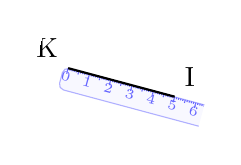
\begin{tikzpicture}[scale=0.28,rotate=-15,every node/.style={scale=1}]

\clip (-1.5,-1.5) rectangle (6.4,1.5);
%%%%%%%%%%%%%%%%%%%%%%%%
%%%%%%%%%%%%%%%%%%%%%%%%
%Début règle !! Si la figure est tournée, il faut
%rajouter l'angle de rotation dans le node des graduation
%pour que les nombres soient écrits correctement
%%%%%%%%%%%%%%%%%%%%%%%%
%%%%%%%%%%%%%%%%%%%%%%%% 

    %Graduation max. de la règle
    \def \Taille {6.5}
    %Définition de l 'angle de rotation de la règle
    \def \Rotation {0}
    %Définition du décalage de la règle
    \def \DecalX {0}
    \def \DecalY {-0.51}
    %Couleur des éléments de la règle (sauf le remplissage)
    \def \RegleColor {blue!60}

\begin{scope}[shift={(\DecalX,\DecalY)},rotate=\Rotation,scale=1]
    % contours de la règle
    \draw[color=\RegleColor, fill =blue!5, opacity=0.5,rounded corners=2pt] (-0.2,0.5) rectangle (\Taille+0.2,-0.5);	%Dont couleur de remplissage
    % graduation 1 mm
    \foreach \a in {0,0.1,...,\Taille}{\draw[color=\RegleColor] (\a,0.5)--(\a,0.42);}
    % graduation 5 mm
    \foreach \a in {0,0.5,...,\Taille}{\draw[color=\RegleColor] (\a,0.42)--(\a,0.35);}
    % graduation et repères 10 mm
    \foreach \a in {0,1,...,\Taille}{\draw[color=\RegleColor] (\a,0.35)--(\a,0.25)
    node[font=\tiny, rotate=\Rotation-15] (\a) at (\a,0.1){\a};}%ici rajouter l'angle de rotation de la figure complète pour que les nombres soient écrits correctement
\end{scope}

%%%%%%%%%%%%%%%%%%%%%%%%
%%%%%%%%%%%%%%%%%%%%%%%%
%Fin de la règle
%%%%%%%%%%%%%%%%%%%%%%%%
%%%%%%%%%%%%%%%%%%%%%%%%

\draw[thick] (0,0) node [above left]{K}--(5,0) node[above right]{I};

\end{tikzpicture} 
